\section{Truck costing and emissions}
\label{sec:costs_emissions}

The long-haul truck simulation model presented in Sader et al. \cite{Sader_2023} is adapted to represent the Tesla Semi. Flexibility is added to the lifecycle emissions and total cost of ownership analysis in the study to represent a range of truck payloads, annual mileage, and charging powers. 

\subsection{Adaptation to the Tesla Semi}

Sader et al. \cite{Sader_2023} developed a detailed physics-based model to simulate the instantaneous power requirements that would be placed on the battery of an electric class 8 sleeper cab truck carrying out the cross-country drivecycle shown in Figure \ref{fig:long_haul_drivecycle}. The drivecycle used in \cite{Sader_2023} specifies the speed and road grade on a second-by-second basis, as shown in Figure \ref{fig:drivecycles}.

\begin{figure}[ht]
    \centering
    \begin{subfigure}[b]{0.49\textwidth}
        \centering
        \includegraphics[width=\textwidth]{figures/long_haul_drivecycle.png}
        \caption{Drivecycle used for the long-haul truck simulation in \cite{Sader_2023}.}
        \label{fig:long_haul_drivecycle}
    \end{subfigure}
    \hfill
    \begin{subfigure}[b]{0.49\textwidth}
        \centering
        \includegraphics[width=\textwidth]{figures/pepsi_3_drive_cycle_24_paper.png}
        \caption{Sample drivecycle from PepsiCo's Tesla Semi pilot}
        \label{fig:sample_pepsico_drivecycle}
    \end{subfigure}
    \caption{Comparison of long-haul drivecycle used in Ref. \cite{Sader_2023} with a sample drivecycle from PepsiCo's 2023 Tesla Semi pilot}
    \label{fig:drivecycles}
\end{figure}

Starting from the \href{https://colab.research.google.com/drive/124rFu_4vHx4cP6SODtdzCxnUmLY50wbW?usp=sharing}{open-source google colab notebook} published as supplementary material with Ref. \cite{Sader_2023}, the model was adapted to represent the Tesla Semi, based on performance data published from three Semis used in a 2023 pilot carried out by PepsiCo in partnership with the \textit{Run on Less - Electric DEPOT demonstration} \cite{NACFE_2023}. 

\subsubsection{Impact of Neglecting Road Grade}

The truck simulation model presented in Ref. \cite{Sader_2023} accounts for the impact of road grade on the instantaneous power demand to the truck battery. However, the drivecycle datasets from the Tesla Semi pilot do not include road grade information. Therefore, prior to adapting the model using these drivecycle datasets, we quantified the impact of neglecting the road grade information in the long-haul drivecycle shown in Figure \ref{fig:long_haul_drivecycle} on the cost and emission results of the original model. 

As shown in Figure \ref{fig:road_grade_comparison}, neglecting road grade results in a 1-3\% underestimate of total cost to society components, and a 2.85-2.95\% underestimate of lifecycle emissions. These systematic effects are well within the uncertainties of other components of the cost and emissions calculations (such as the capital and electricity costs, grid emission intensity), and are thus considered negligible. 

\begin{figure}[ht]
    \centering
    \begin{subfigure}[b]{0.54\textwidth}
        \centering
        \includegraphics[width=\textwidth]{figures/results_comparison_costing.png}
        \caption{Total cost of ownership}
        \label{fig:results_comparison_costing}
    \end{subfigure}
    \hfill
    \begin{subfigure}[b]{0.44\textwidth}
        \centering
        \includegraphics[width=\textwidth]{figures/results_comparison_emissions.png}
        \caption{Lifecycle emissions}
        \label{fig:results_comparison_emissions}
    \end{subfigure}
    \caption{Impact of neglecting road grade on major components of total cost of ownership (left) and lifecycle emissions (right) calculations using the model presented in Sader et al. \cite{Sader_2023}}
    \label{fig:road_grade_comparison}
\end{figure}


\subsubsection{Analysis of Tesla Semi Performance Data}

\subsubsubsection{Drivecycle Extraction}

Twenty drivecycles are extracted from second-by-second performance data collected by onboard Geotab GO9 devices \cite{Geotab_2024} installed on the three trucks involved in PepsiCo's 2023 Tesla Semi pilot \cite{NACFE_2023}. Table \ref{tab:nacfe_performance_data} summarizes the performance data information used in this analysis. An individual drivecycles is defined as a period between charging events during which the battery is registered as either losing energy to driving or gaining it to regenerative braking. The green bands in Figure \ref{fig:pepsi_3_drivecycles} represent individual drivecycles identified in the data collected from one of the three trucks. 

\begin{table}[ht]
\centering
\begin{tabular}{P{4cm}P{10cm}} % Adjust the column widths as needed
\toprule % Thicker top line
\textbf{Information} & \textbf{Description} \\ \midrule % Midrule for under header
Timestamp & Timestamp, down to 1-second precision. Adjacent timestamps are typically separated by 1 second, but longer breaks occur occasionally. \\
\midrule % Thin line between rows
Speed & Moving speed of the truck, in miles per hour (mph) \\
\midrule
Distance & Cumulative distance traveled (miles) \\
\midrule
State of Charge & Battery state of charge (\%) \\
\midrule
Energy Type & Mode in which the battery is accumulating or losing energy. Data from the Semis included following modes: \verb|driving_energy| (energy lost while driving), \verb|energy_regen| (energy gained from regenerative braking), and \verb|energy_from_dc_charger| (energy gained from DC charging). \\
\midrule
Accumulated Battery Energy & Battery energy accumulated (if Energy Type is \verb|energy_from_dc_charger| or \verb|energy_regen|) or lost (if Energy Type is \verb|driving_energy|) \\
\bottomrule % Thicker bottom line
\end{tabular}
\caption{Summary of information from Tesla Semi pilot performance data used in the analysis. The data was collected from three trucks involved in the pilot, and published by NACFE as part of the \textit{Run on Less - Electric DEPOT demonstration} \cite{NACFE_2023}.}
\label{tab:nacfe_performance_data}
\end{table}

\begin{figure}[ht]
        \centering
        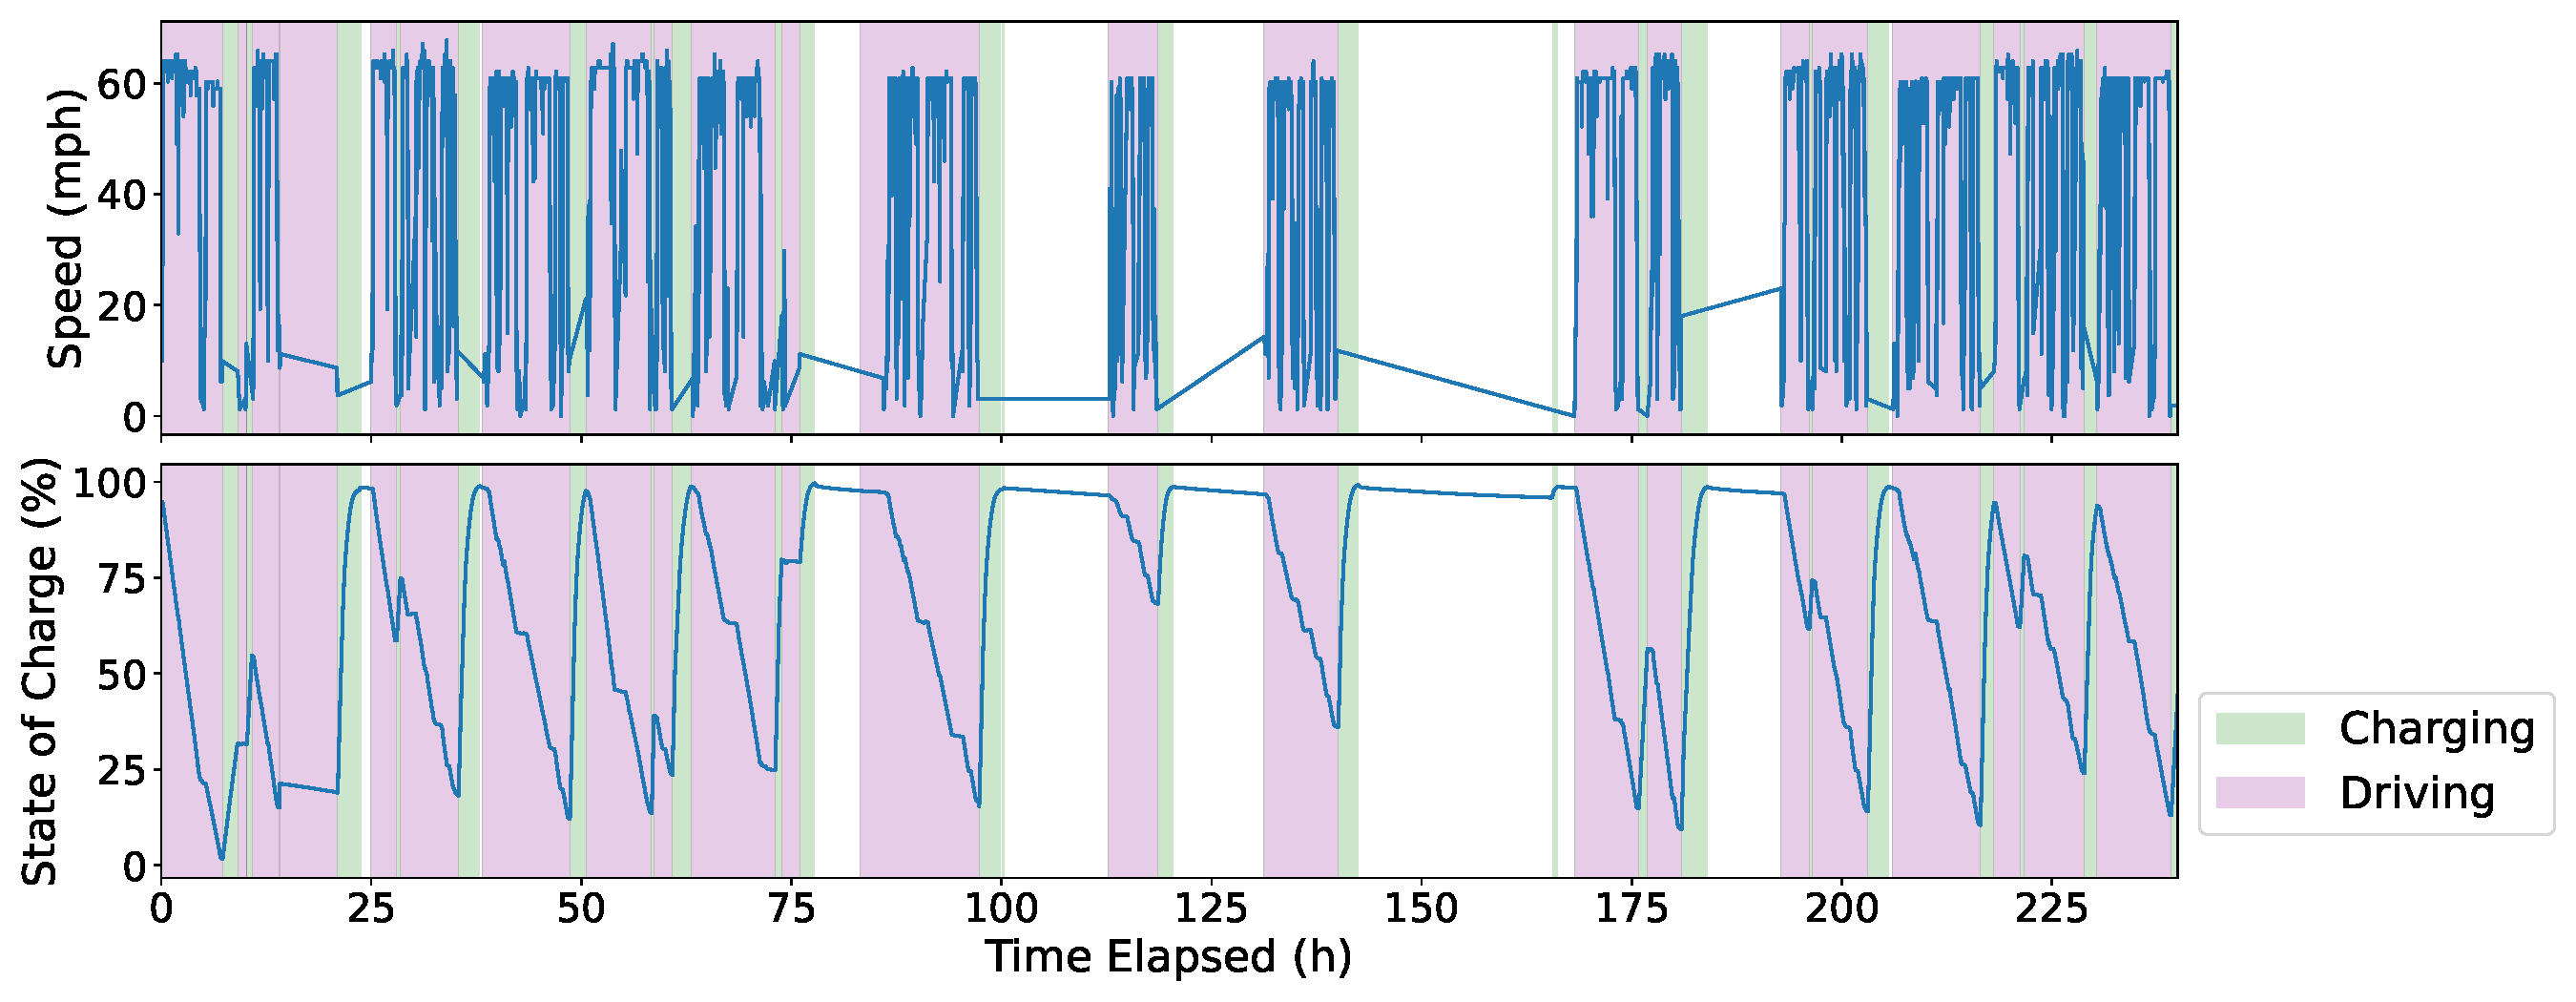
\includegraphics[width=\textwidth]{figures/pepsi_3_speed_vs_time.png}
        \caption{Driving and charging periods identified in the geotab data collected from the \textit{Pepsi 3} truck}
        \label{fig:pepsi_3_drivecycles}
\end{figure}

\subsubsubsection{Performance Parameter Evaluation}

The performance data is used to evaluate the battery capacity within each charging period, and the vehicle range and energy economy within each drivecycle.

Within a given charging period, the battery capacity is evaluated by fitting a quadratic function to the accumulated battery energy as a function of the reported state of charge using least squares regression, and extrapolating to the full charge range.

In principle, the battery energy would be expected to increase linearly with the state of charge, but in practice a quadratic fit is generally seen to yield significant improvement relative to linear, as measured by root mean squared error (RMSE). This is illustrated for a sample charging event in Figure \ref{fig:charging_fits}.

\begin{figure}[ht]
    \centering
    \begin{subfigure}[b]{0.48\textwidth}
        \centering
        \includegraphics[width=\textwidth]{figures/pepsi_1_battery_soc_vs_energy_event_11_linearfit.png}
        \caption{Linear fit}
        \label{fig:charging_linear_fit}
    \end{subfigure}
    \hfill
    \begin{subfigure}[b]{0.48\textwidth}
        \centering
        \includegraphics[width=\textwidth]{figures/pepsi_1_battery_soc_vs_energy_event_11_quadfit.png}
        \caption{Quadratic fit}
        \label{fig:charging_quad_fit}
    \end{subfigure}
    \caption{Comparison of linear and quadratic fits to the battery energy as a function of state of charge for a sample charging event collected from the \textit{Pepsi 1} truck.}
    \label{fig:charging_fits}
\end{figure}

For each fit, the battery size was extrapolated from the fitting function $f_\text{fit}$ as:

\begin{equation}
    \text{Battery size}_\text{charging event i} = f_\text{fit, i}(\text{State of charge = 100\%}) - f_\text{fit, i}(\text{State of charge = 0\%})
\end{equation}

For a given truck, the battery size is estimated using the weighted mean over all charging events that satisfy the criteria outlined in Table \ref{tab:charging_event_criteria}:

\begin{equation}
    \overline{\text{Battery size}}_\text{truck j} = \frac{\sum_\text{event i}^\text{N} (\text{Battery size}_i/\sigma_i)^2}{\sum_\text{event i}^\text{N}(1/\sigma_i)}
\end{equation}

where $N$ is the total number of charging events that pass the criteria for the given truck, and $\sigma_i$ is the uncertainty in the evaluated battery size for charging event $i$ in truck $j$. The uncertainty $\delta(\text{Battery size}_\text{truck j})$ is evaluated using the weighted standard deviation:

\begin{equation}
    \delta(\text{Battery size}_\text{truck j}) = \sqrt{\frac{\sum (\frac{1}{\sigma_i^2}) (\text{Battery size}_i - \overline{\text{Battery size}}_\text{truck j})^2}{\sum \frac{1}{\sigma_i}^2}}
\end{equation}

Battery sizes were evaluated using this methodology for charging events with at least 10 datapoints that covered at least 50\% of the battery's state of charge range.

Figure \ref{fig:battery_capacity_summary} shows the extrapolated battery capacities for a sample truck and the weighted mean over all drivecycles. The results are summarized in Table \ref{tab:battery_capacity_summary}, with a weighted mean battery capacity of (823 $\pm$ 2) kWh over all Semi trucks.

\begin{figure}[ht]
        \centering
        \includegraphics[width=0.6\textwidth]{figures/pepsi_1_battery_capacity_summary.png}
        \caption{Summary of battery capacity estimates extrapolated from quadratic fits to battery energy as a function of state of charge for the \textit{Pepsi 1} truck}
        \label{fig:battery_capacity_summary}
\end{figure}

\begin{table}[ht]
\centering
\begin{tabular}{P{4cm}P{6cm}} % Adjust the column widths as needed
\toprule % Thicker top line
\textbf{Truck} & \textbf{Battery capacity (kWh)} \\ \midrule % Midrule for under header
Pepsi 1 & 822 $\pm$ 3 \\
\midrule
Pepsi 2 & 825 $\pm$ 7 \\
\midrule
Pepsi 3 & 827 $\pm$ 6 \\
\midrule
Combined & 823 $\pm$ 2 \\
\bottomrule % Thicker bottom line
\end{tabular}
\caption{Summary of battery capacity estimates for each Tesla Semi in the pilot, obtained using weighted mean over all charging events passing the criteria in Table \ref{tab:charging_event_criteria}}
\label{tab:battery_capacity_summary}
\end{table}

Within a given drivecycle, the range is extrapolated using a linear fit to the distance traveled as a function of state of charge, using a procedure analogous to that presented above to evaluate battery sizes. The energy economy for a given drivecycle is evaluated as:

\begin{equation}
    \text{Energy economy}_\text{drivecycle i, truck j} = \frac{\text{DoD}_i * \text{Battery size}_\text{truck j}}{\text{Distance Traveled}_i}
\end{equation}

where the depth of discharge DoD is the relative loss of battery charge over the full drivecycle: $\text{DoD} = (\text{state of charge})_\text{init} - \text{state of charge})_\text{final}) / 100\%$.

The distance vs. charge curves are generally found to fall into two classes, extreme examples of which are shown in Figure \ref{fig:distance_vs_soc}. The first class (``linear") is well-represented by a linear fit, whereas the second class (``non-linear") exhibits strong non-linearities. 

\begin{figure}[ht]
    \centering
    \begin{subfigure}[b]{0.48\textwidth}
        \centering
        \includegraphics[width=\textwidth]{figures/distance_vs_soc_linear.png}
        \caption{Linear drivecycle}
        \label{fig:distance_vs_soc_linear}
    \end{subfigure}
    \hfill
    \begin{subfigure}[b]{0.48\textwidth}
        \centering
        \includegraphics[width=\textwidth]{figures/distance_vs_soc_nonlinear.png}
        \caption{Nonlinear}
        \label{fig:distance_vs_soc_nonlinear}
    \end{subfigure}
    \caption{Sample drivecycles showing speed and distance traveled as a function of state of charge. The left-hand drivecycle is classified as ``linear", and the right-hand as ``nonlinear" on the basis of their linear fit RMSE.}
    \label{fig:distance_vs_soc}
\end{figure}

It is assumed that the non-linear curves represent roundtrips from Sacramento, CA to Reno, NV discussed in Ref. \cite{NACFE_2023}, which cover mountainous terrain that would be expected to incur significant variations on power demand to the battery, including regenerative braking on downhill sections. Conversely, the curves with strong linearity are assumed to represent operations in the vicinity of Sacramento, within the flat Central Valley region of California. 

The drivecycles are classified as linear or non-linear according to the RMSE of their linear fit. Figure \ref{fig:rmse_dist} shows the distribution of RMSE for linear fits over all drivecycles. A cutoff of 5 is placed to mark the boundary below which minimal nonlinear behavior is observed. Figure \ref{fig:distance_vs_soc_cutoff} shows a sample of drivecycles with RMSE near this cutoff. 

\begin{figure}[ht]
        \centering
        \includegraphics[width=0.5\textwidth]{figures/all_RMSE.png}
        \caption{Distribution of RMSE for linear fits to the distance traveled as a function of battery state of charge over all drivecycles. The red dashed line shows the placement of the RMSE cutoff for the ``linear" classification.}
        \label{fig:rmse_dist}
\end{figure}

\begin{figure}[ht]
    \centering
    \begin{subfigure}[b]{0.48\textwidth}
        \centering
        \includegraphics[width=\textwidth]{figures/distance_vs_soc_below_cutoff.png}
        \caption{RMSE$ = 4.88$ (linear)}
        \label{fig:distance_vs_soc_below_cutoff}
    \end{subfigure}
    \hfill
    \begin{subfigure}[b]{0.48\textwidth}
        \centering
        \includegraphics[width=\textwidth]{figures/distance_vs_soc_above_cutoff.png}
        \caption{RMSE$ = 5.49$ (non-linear)}
        \label{fig:distance_vs_soc_above_cutoff}
    \end{subfigure}
    \caption{Sample drivecycles showing speed and distance traveled as a function of state of charge. The left-hand drivecycle has an RMSE falling just below the linearity cutoff of 5 (so is classified as ``linear), and the right-hand drivecycle falls just above the cutoff.}
    \label{fig:distance_vs_soc_cutoff}
\end{figure}

\subsubsection{Model Parameter Modifications}

Analysis of the Tesla 

\subsubsection{Payload Evaluation}

\subsubsection{Payload Dependence of Energy Economy}

\subsubsection{Vehicle Model Adaptations}

\subsubsection{Adaptations for Lifecycle Costing and Emissions}


